\documentclass[a4paper,12pt,twoside]{memoir}

% Castellano
\usepackage[spanish,es-tabla]{babel}
\selectlanguage{spanish}
\usepackage[utf8]{inputenc}
\usepackage[T1]{fontenc}
\usepackage{lmodern} % Scalable font
\usepackage{microtype}
\usepackage{placeins}
\usepackage{amssymb}

\RequirePackage{booktabs}
\RequirePackage[table]{xcolor}
\RequirePackage{xtab}
\RequirePackage{multirow}

% Links
\PassOptionsToPackage{hyphens}{url}\usepackage[colorlinks]{hyperref}
\hypersetup{
	allcolors = {blue}
}

% Ecuaciones
\usepackage{amsmath}

% Rutas de fichero / paquete
\newcommand{\ruta}[1]{{\sffamily #1}}

% Párrafos
\nonzeroparskip

% Huérfanas y viudas
\widowpenalty100000
\clubpenalty100000

% Imágenes

% Comando para insertar una imagen en un lugar concreto.
% Los parámetros son:
% 1 --> Ruta absoluta/relativa de la figura
% 2 --> Texto a pie de figura
% 3 --> Tamaño en tanto por uno relativo al ancho de página
\usepackage{graphicx}
\newcommand{\imagen}[3]{
	\begin{figure}[!h]
		\centering
		\includegraphics[width=#3\textwidth]{#1}
		\caption{#2}\label{fig:#1}
	\end{figure}
	\FloatBarrier
}

% Comando para insertar una imagen sin posición.
% Los parámetros son:
% 1 --> Ruta absoluta/relativa de la figura
% 2 --> Texto a pie de figura
% 3 --> Tamaño en tanto por uno relativo al ancho de página
\newcommand{\imagenflotante}[3]{
	\begin{figure}
		\centering
		\includegraphics[width=#3\textwidth]{#1}
		\caption{#2}\label{fig:#1}
	\end{figure}
}

% El comando \figura nos permite insertar figuras comodamente, y utilizando
% siempre el mismo formato. Los parametros son:
% 1 --> Porcentaje del ancho de página que ocupará la figura (de 0 a 1)
% 2 --> Fichero de la imagen
% 3 --> Texto a pie de imagen
% 4 --> Etiqueta (label) para referencias
% 5 --> Opciones que queramos pasarle al \includegraphics
% 6 --> Opciones de posicionamiento a pasarle a \begin{figure}
\newcommand{\figuraConPosicion}[6]{%
  \setlength{\anchoFloat}{#1\textwidth}%
  \addtolength{\anchoFloat}{-4\fboxsep}%
  \setlength{\anchoFigura}{\anchoFloat}%
  \begin{figure}[#6]
    \begin{center}%
      \Ovalbox{%
        \begin{minipage}{\anchoFloat}%
          \begin{center}%
            \includegraphics[width=\anchoFigura,#5]{#2}%
            \caption{#3}%
            \label{#4}%
          \end{center}%
        \end{minipage}
      }%
    \end{center}%
  \end{figure}%
}

%
% Comando para incluir imágenes en formato apaisado (sin marco).
\newcommand{\figuraApaisadaSinMarco}[5]{%
  \begin{figure}%
    \begin{center}%
    \includegraphics[angle=90,height=#1\textheight,#5]{#2}%
    \caption{#3}%
    \label{#4}%
    \end{center}%
  \end{figure}%
}
% Para las tablas
\newcommand{\otoprule}{\midrule [\heavyrulewidth]}
%
% Nuevo comando para tablas pequeñas (menos de una página).
\newcommand{\tablaSmall}[5]{%
 \begin{table}
  \begin{center}
   \rowcolors {2}{gray!35}{}
   \begin{tabular}{#2}
    \toprule
    #4
    \otoprule
    #5
    \bottomrule
   \end{tabular}
   \caption{#1}
   \label{tabla:#3}
  \end{center}
 \end{table}
}

%
% Nuevo comando para tablas pequeñas (menos de una página).
\newcommand{\tablaSmallSinColores}[5]{%
 \begin{table}[H]
  \begin{center}
   \begin{tabular}{#2}
    \toprule
    #4
    \otoprule
    #5
    \bottomrule
   \end{tabular}
   \caption{#1}
   \label{tabla:#3}
  \end{center}
 \end{table}
}

\newcommand{\tablaApaisadaSmall}[5]{%
\begin{landscape}
  \begin{table}
   \begin{center}
    \rowcolors {2}{gray!35}{}
    \begin{tabular}{#2}
     \toprule
     #4
     \otoprule
     #5
     \bottomrule
    \end{tabular}
    \caption{#1}
    \label{tabla:#3}
   \end{center}
  \end{table}
\end{landscape}
}

%
% Nuevo comando para tablas grandes con cabecera y filas alternas coloreadas en gris.
\newcommand{\tabla}[6]{%
  \begin{center}
    \tablefirsthead{
      \toprule
      #5
      \otoprule
    }
    \tablehead{
      \multicolumn{#3}{l}{\small\sl continúa desde la página anterior}\\
      \toprule
      #5
      \otoprule
    }
    \tabletail{
      \hline
      \multicolumn{#3}{r}{\small\sl continúa en la página siguiente}\\
    }
    \tablelasttail{
      \hline
    }
    \bottomcaption{#1}
    \rowcolors {2}{gray!35}{}
    \begin{xtabular}{#2}
      #6
      \bottomrule
    \end{xtabular}
    \label{tabla:#4}
  \end{center}
}

%
% Nuevo comando para tablas grandes con cabecera.
\newcommand{\tablaSinColores}[6]{%
  \begin{center}
    \tablefirsthead{
      \toprule
      #5
      \otoprule
    }
    \tablehead{
      \multicolumn{#3}{l}{\small\sl continúa desde la página anterior}\\
      \toprule
      #5
      \otoprule
    }
    \tabletail{
      \hline
      \multicolumn{#3}{r}{\small\sl continúa en la página siguiente}\\
    }
    \tablelasttail{
      \hline
    }
    \bottomcaption{#1}
    \begin{xtabular}{#2}
      #6
      \bottomrule
    \end{xtabular}
    \label{tabla:#4}
  \end{center}
}

%
% Nuevo comando para tablas grandes sin cabecera.
\newcommand{\tablaSinCabecera}[5]{%
  \begin{center}
    \tablefirsthead{
      \toprule
    }
    \tablehead{
      \multicolumn{#3}{l}{\small\sl continúa desde la página anterior}\\
      \hline
    }
    \tabletail{
      \hline
      \multicolumn{#3}{r}{\small\sl continúa en la página siguiente}\\
    }
    \tablelasttail{
      \hline
    }
    \bottomcaption{#1}
  \begin{xtabular}{#2}
    #5
   \bottomrule
  \end{xtabular}
  \label{tabla:#4}
  \end{center}
}



\definecolor{cgoLight}{HTML}{EEEEEE}
\definecolor{cgoExtralight}{HTML}{FFFFFF}

%
% Nuevo comando para tablas grandes sin cabecera.
\newcommand{\tablaSinCabeceraConBandas}[5]{%
  \begin{center}
    \tablefirsthead{
      \toprule
    }
    \tablehead{
      \multicolumn{#3}{l}{\small\sl continúa desde la página anterior}\\
      \hline
    }
    \tabletail{
      \hline
      \multicolumn{#3}{r}{\small\sl continúa en la página siguiente}\\
    }
    \tablelasttail{
      \hline
    }
    \bottomcaption{#1}
    \rowcolors[]{1}{cgoExtralight}{cgoLight}

  \begin{xtabular}{#2}
    #5
   \bottomrule
  \end{xtabular}
  \label{tabla:#4}
  \end{center}
}



\graphicspath{ {./img/} }

% Capítulos
\chapterstyle{bianchi}
\newcommand{\capitulo}[2]{
	\setcounter{chapter}{#1}
	\setcounter{section}{0}
	\setcounter{figure}{0}
	\setcounter{table}{0}
	\chapter*{\thechapter.\enskip #2}
	\addcontentsline{toc}{chapter}{\thechapter.\enskip #2}
	\markboth{#2}{#2}
}

% Apéndices
\renewcommand{\appendixname}{Apéndice}
\renewcommand*\cftappendixname{\appendixname}

\newcommand{\apendice}[1]{
	%\renewcommand{\thechapter}{A}
	\chapter{#1}
}

\renewcommand*\cftappendixname{\appendixname\ }

% Formato de portada
\makeatletter
\usepackage{xcolor}
\newcommand{\tutor}[1]{\def\@tutor{#1}}
\newcommand{\tutors}[1]{\def\@tutors{#1}}
\newcommand{\course}[1]{\def\@course{#1}}
\definecolor{cpardoBox}{HTML}{E6E6FF}
\def\maketitle{
  \null
  \thispagestyle{empty}
  % Cabecera ----------------
\noindent\includegraphics[width=\textwidth]{cabecera}\vspace{1cm}%
  \vfill
  % Título proyecto y escudo informática ----------------
  \colorbox{cpardoBox}{%
    \begin{minipage}{.8\textwidth}
      \vspace{.5cm}\Large
      \begin{center}
      \textbf{TFG del Grado en Ingeniería Informática}\vspace{.6cm}\\
      \textbf{\LARGE\@title{}}
      \end{center}
      \vspace{.2cm}
    \end{minipage}

  }%
  \hfill\begin{minipage}{.20\textwidth}
    \includegraphics[width=\textwidth]{escudoInfor}
  \end{minipage}
  \vfill
  % Datos de alumno, curso y tutores ------------------
  \begin{center}%
  {%
    \noindent\LARGE
    Presentado por \@author{}\\ 
    en Universidad de Burgos --- \@date{}\\
    Tutor: \@tutor{}\\
	Tutor: \@tutors{}\\
  }%
  \end{center}%
  \null
  \cleardoublepage
  }
\makeatother

\newcommand{\nombre}{José Luis Caballero Martínez-Quintanilla} %%% cambio de comando

% Datos de portada
\title{Diseño de un sistema económico IoT de monitorización de invernaderos de cannabis medicinal}
\author{\nombre}
\tutor{Alejandro Merino Gómez}
\tutors{Carlos Cambra Baseca}
\date{16 de febrero de 2024}

\begin{document}

\maketitle


\newpage\null\thispagestyle{empty}\newpage


%%%%%%%%%%%%%%%%%%%%%%%%%%%%%%%%%%%%%%%%%%%%%%%%%%%%%%%%%%%%%%%%%%%%%%%%%%%%%%%%%%%%%%%%
\thispagestyle{empty}


\noindent\includegraphics[width=\textwidth]{cabecera}\vspace{1cm}

\noindent D. Alejandro Merino Gómez, profesor del departamento de Digitalización, área de Systems Engineering and Automation y D. Carlos Cambra Baseca, profesor del departamento de Digitalización del área de Computer Science and Artificial Intelligence, 

\noindent Exponen:

\noindent Que el alumno D. \nombre, con DNI 48471169-A, ha realizado el Trabajo final de Grado en Ingeniería Informática titulado Diseño de un sistema económico IoT de monitorización de invernaderos de cannabis medicinal. 

\noindent Y que dicho trabajo ha sido realizado por el alumno bajo la dirección del que suscribe, en virtud de lo cual se autoriza su presentación y defensa.

\begin{center} %\large
En Burgos, {\large 16 de febrero de 2024}
\end{center}

\vfill\vfill\vfill

% Author and supervisor
\begin{minipage}{0.45\textwidth}
\begin{flushleft} %\large
Vº. Bº. del Tutor:\\[2cm]
D. Merino Gómez, Alejandro
\end{flushleft}
\end{minipage}
\hfill
\begin{minipage}{0.45\textwidth}
\begin{flushleft} %\large
Vº. Bº. del co-tutor:\\[2cm]
D. Cambra Baseca, Carlos 
\end{flushleft}
\end{minipage}
\hfill

\vfill

% para casos con solo un tutor comentar lo anterior
% y descomentar lo siguiente
%Vº. Bº. del Tutor:\\[2cm]
%D. nombre tutor


\newpage\null\thispagestyle{empty}\newpage




\frontmatter

% Abstract en castellano
\renewcommand*\abstractname{Resumen}
\begin{abstract}
El presente trabajo de fin de grado aborda el diseño de un sistema económico basado en el Internet de las cosas (IoT) para la monitorización de invernaderos destinados al cultivo de cannabis medicinal. El objetivo principal es mejorar la eficiencia y la calidad del cultivo mediante la implementación de sensores y dispositivos conectados que permitan la recolección y análisis de datos en tiempo real.

El hardware seleccionado para este proyecto incluye la Raspberry Pi Pico W como unidad central, una pantalla OLED 128x64 para la visualización de información, el sensor DHT22 para la medición de la temperatura y humedad ambiente, el sensor BH1750 para evaluar la intensidad lumínica, y un sensor de humedad de suelo para monitorear las condiciones de la tierra.

A lo largo del trabajo, se detalla el proceso de integración de estos componentes, se describen las tecnologías utilizadas para la comunicación y el manejo de datos, y se presenta la interfaz de usuario diseñada para la visualización de información relevante. Se destacan también las consideraciones económicas que han llevado a la elección de cada componente, buscando una solución asequible sin comprometer la calidad de los resultados.

Los resultados obtenidos demuestran la viabilidad y eficacia del sistema propuesto, ofreciendo a los agricultores de cannabis medicinal un instrumento práctico y accesible para mejorar la gestión de sus invernaderos. Este trabajo contribuye al campo emergente de la agricultura inteligente y sostenible, abriendo posibilidades para futuras investigaciones y aplicaciones en el ámbito de la monitorización agrícola basada en IoT.

\end{abstract}

\renewcommand*\abstractname{Descriptores}
\begin{abstract}
Raspberry Pi Pico W, Micropython, Autónomo, Sistema Domótico, Bot, Telegram, Python, MQTT, SQL \ldots
\end{abstract}

\clearpage

% Abstract en inglés
\renewcommand*\abstractname{Abstract}
\begin{abstract}
This project deals with the design of an economic system based on the Internet of Things (IoT) for the monitoring of greenhouses for the cultivation of medical cannabis. The main objective is to improve the efficiency and quality of the crop through the implementation of sensors and connected devices that allow the collection and analysis of data in real time.

The hardware selected for this project includes the Raspberry Pi Pico W as the central unit, a 128x64 OLED screen for displaying information, the DHT22 sensor for measuring ambient temperature and humidity, the BH1750 sensor for evaluating light intensity, and a soil moisture sensor for monitoring soil conditions.

Throughout the paper, the integration process of these components is detailed, the technologies used for communication and data management are described, and the user interface designed for the visualization of relevant information is presented. It also highlights the economic considerations that led to the choice of each component, seeking an affordable solution without compromising the quality of the results.

The results obtained demonstrate the feasibility and effectiveness of the proposed system, offering medical cannabis farmers a practical and accessible tool to improve the management of their greenhouses. This work contributes to the emerging field of smart and sustainable agriculture, opening possibilities for future research and applications in the field of IoT-based agricultural monitoring.
\end{abstract}

\renewcommand*\abstractname{Keywords}
\begin{abstract}
Raspberry Pi Pico W, Micropython, Autonomous, Domotic System, Bot, Telegram, Python, MQTT, SQL\ldots
\end{abstract}

\clearpage

% Indices
\tableofcontents

\clearpage

\listoffigures

\clearpage

\listoftables
\clearpage

\mainmatter
\capitulo{1}{Introducción}

El panorama en constante cambio de la industria del cannabis medicinal ha generado una creciente necesidad de optimizar los métodos de cultivo para garantizar la consistencia y calidad de los productos. En este contexto, el Internet de las cosas (IoT) emerge como una herramienta clave para transformar la gestión de invernaderos, permitiendo una monitorización en tiempo real y decisiones informadas por parte de los agricultores.

Este trabajo se centra en el diseño de un sistema asequible de monitorización basado en IoT para invernaderos de cannabis medicinal. La elección de hardware, liderada por la Raspberry Pi Pico W como unidad central, se fundamenta en la capacidad de esta plataforma para equilibrar eficiencia y costos. Sensores especializados, como el DHT22 para temperatura y humedad, el BH1750 para intensidad lumínica, y un sensor de humedad de suelo, complementan la infraestructura del sistema.

Más allá de la mejora en la eficiencia del cultivo de cannabis medicinal, este proyecto busca situarse en la vanguardia de la agricultura inteligente y sostenible. La combinación de IoT con prácticas agrícolas avanzadas tiene el potencial de transformar radicalmente la forma en que se gestionan los cultivos, promoviendo la sostenibilidad y ofreciendo una solución práctica para agricultores de diversos niveles de recursos.

En resumen, este trabajo se adentra en el diseño de un sistema completo y accesible para la monitorización de invernaderos, utilizando la innovación tecnológica como catalizador para mejorar la calidad de los cultivos y contribuir al avance de la agricultura moderna.

\capitulo{2}{Objetivos del proyecto}
%Este apartado explica de forma precisa y concisa cuales son los objetivos que se persiguen con la realización del proyecto. Se puede distinguir entre los objetivos marcados por los requisitos del software a construir y los objetivos de carácter técnico que plantea a la hora de llevar a la práctica el proyecto.
\section{Objetivos del Software}
\begin{itemize}
\item \textbf{Desarrollo del Sistema de Adquisición de Datos:}
Implementar un sistema eficiente de adquisición de datos que pueda recopilar información precisa proveniente de los sensores (DHT22, BH1750, sensor de humedad de suelo) instalados en el invernadero.
\item \textbf{Diseño de la Interfaz de Usuario:}
Desarrollar una interfaz de usuario intuitiva y fácil de usar, que permita a los usuarios visualizar en tiempo real los datos recopilados y tomar decisiones informadas sobre el control del entorno del invernadero.
\item \textbf{Implementación de Protocolos de Comunicación:}
Establecer protocolos de comunicación eficientes para la transmisión de datos entre los sensores y la Raspberry Pi Pico W, así como para la conexión con otros dispositivos o sistemas externos si es necesario.
\end{itemize}
\pagebreak

\section{Objetivos Técnicos}
\begin{itemize}
\item \textbf{Integración de Hardware:} 
Seleccionar, configurar e integrar de manera óptima el hardware necesario (Raspberry Pi Pico W, pantalla OLED 128x64, sensores) para garantizar la estabilidad y la eficacia del sistema.

\item \textbf{Eficiencia Energética:}
Implementar estrategias de programación y configuración de hardware que optimicen el consumo de energía, asegurando una operación sostenible del sistema en entornos con recursos limitados. Precisamente la Raspberry Pi Pico W es conocida por su bajo consumo energético.

\item \textbf{Validación en Entorno Real:}
Realizar pruebas exhaustivas del sistema en un entorno de cultivo de cannabis medicinal real, evaluando su rendimiento, confiabilidad y adaptabilidad a condiciones variables.

\item \textbf{Consideraciones Económicas:}
Evaluar y optimizar los costos asociados al desarrollo e implementación del sistema, garantizando la viabilidad económica para agricultores de diferentes escalas y recursos.

\item \textbf{Documentación Completa:}
Generar una documentación detallada que abarque el diseño, la implementación y la configuración del sistema, facilitando la comprensión y la replicación por parte de otros interesados.
Estos objetivos, tanto del software como técnicos, se plantean con el propósito de cumplir con los requisitos del proyecto y garantizar la efectividad y utilidad del sistema de monitorización propuesto para invernaderos de cannabis medicinal.
\end{itemize}

\capitulo{3}{Conceptos teóricos}

%En aquellos proyectos que necesiten para su comprensión y desarrollo de unos conceptos teóricos de una determinada materia o de un determinado dominio de conocimiento, debe existir un apartado que sintetice dichos conceptos.

%Algunos conceptos teóricos de \LaTeX{} \footnote{Créditos a los proyectos de Álvaro López Cantero: Configurador de Presupuestos y Roberto Izquierdo Amo: PLQuiz}.

%\section{Referencias}
%Las referencias se incluyen en el texto usando cite~\cite{wiki:latex}. Para citar webs, artículos o libros~\cite{koza92}, si se desean citar más de uno en el mismo lugar~\cite{bortolot2005, koza92}.

%\imagen{escudoInfor}{Autómata para una expresión vacía}{.5} %imagenes
	
%\section{Tablas}
%Igualmente se pueden usar los comandos específicos de \LaTeX o bien usar alguno de los comandos de la plantilla.
%\tablaSmall{Herramientas y tecnologías utilizadas en cada parte del proyecto}{l c c c c}{herramientasportipodeuso}
%{ \multicolumn{1}{l}{Herramientas} & App AngularJS & API REST & BD & Memoria \\}{ 
%HTML5 & X & & &\\
%CSS3 & X & & &\\
%BOOTSTRAP & X & & &\\
%JavaScript & X & & &\\
%AngularJS & X & & &\\
%Bower & X & & &\\
%PHP & & X & &\\
%Karma + Jasmine & X & & &\\
%Slim framework & & X & &\\
%Idiorm & & X & &\\
%Composer & & X & &\\
%JSON & X & X & &\\
%PhpStorm & X & X & &\\
%MySQL & & & X &\\
%PhpMyAdmin & & & X &\\
%Git + BitBucket & X & X & X & X\\
%Mik\TeX{} & & & & X\\
%\TeX{}Maker & & & & X\\
%Astah & & & & X\\
%Balsamiq Mockups & X & & &\\
%VersionOne & X & X & X & X\\
%} 
\section{Internet de las cosas (IoT)}
El Internet de las cosas (IoT) se refiere a la red de dispositivos físicos que están integrados con tecnología, software, sensores y conectividad de red para recopilar y compartir datos. Estos dispositivos, también llamados \textbf{objetos inteligentes}  o \textbf{dispositivos conectados}, pueden interactuar entre sí y con sistemas informáticos en red para realizar tareas específicas, recopilar información y ofrecer funcionalidades avanzadas.

Características clave del IoT:
\begin{itemize}
\item \textbf{Conectividad:}
Los dispositivos IoT están equipados con tecnologías de comunicación, como Wi-Fi, Bluetooth, Zigbee o incluso 5G, que les permiten conectarse a redes y compartir datos.

\item \textbf{Sensores y Actuadores:}
Los dispositivos IoT suelen estar equipados con sensores para recopilar datos del entorno circundante. Además, algunos dispositivos también incorporan actuadores que les permiten realizar acciones físicas en respuesta a comandos.

\item \textbf{Inteligencia y Procesamiento de Datos:}
Muchos dispositivos IoT cuentan con capacidad de procesamiento local o dependen de la nube para analizar y procesar datos recopilados. La inteligencia artificial y el aprendizaje automático también se aplican para extraer información significativa de grandes conjuntos de datos.

\item \textbf{Interconexión:}
La capacidad de interconectar dispositivos IoT permite que trabajen juntos de manera coordinada, compartiendo información y actuando en función de datos colectivos.

\item \textbf{Aplicaciones Diversas:}
El IoT se aplica en una amplia variedad de campos, como la agricultura inteligente, la salud, la domótica, la industria manufacturera, la logística y más. Esto permite la automatización y mejora de procesos en diversas industrias.

\item \textbf{Seguridad y Privacidad:}
Dado que los dispositivos IoT manejan datos sensibles, la seguridad y la privacidad son aspectos críticos. Se implementan medidas de seguridad para proteger la integridad y la confidencialidad de los datos transmitidos y almacenados.

El Internet de las cosas tiene un impacto significativo en la forma en que interactuamos con el entorno, mejorando la eficiencia, la toma de decisiones y la calidad de vida. A medida que la tecnología avanza, el alcance y la influencia del IoT continúan expandiéndose, creando un ecosistema cada vez más interconectado.
\end{itemize}
\section{Raspberry Pi Pico W}
La Raspberry Pi Pico W~\cite{misc:RPiPicoW} es una placa de desarrollo de bajo costo que combina versatilidad y conectividad inalámbrica. Se elige como unidad central para el sistema, actuando como el cerebro que controla y coordina la recopilación y transmisión de datos.

\section{MicroPython}
MicroPython~\cite{wiki:micropython} es una implementación del lenguaje de programación Python diseñada para sistemas embebidos y microcontroladores como la Raspberry Pi Pico W. Permite una programación sencilla y eficiente de la unidad central, facilitando el desarrollo de aplicaciones en entornos limitados.

\section{GPIO}\label{concepto:GPIO}
GPIO~\cite{misc:gpio}, por sus siglas en inglés, General Purpose Input/Output, se refiere a los pines de propósito general presentes en microcontroladores y sistemas embebidos. Estos pines son versátiles y pueden configurarse tanto como entradas como salidas, permitiendo la interacción del microcontrolador con el entorno externo.
\begin{itemize}
	\item \textbf{Entradas (Input):} En modo de entrada, un pin GPIO puede recibir señales eléctricas del exterior, como las provenientes de sensores o interruptores. Estos pines detectan y leen el estado de la señal, que puede ser alto (1) o bajo (0), dependiendo de la presencia de voltaje.

	\item \textbf{Salidas (Output):} En modo de salida, un pin GPIO puede enviar señales eléctricas al exterior, como las necesarias para controlar actuadores, LEDs u otros dispositivos. El microcontrolador puede controlar el estado del pin, estableciendo un voltaje alto o bajo según sea necesario.
\end{itemize}
La flexibilidad de los pines GPIO permite a los desarrolladores adaptar el comportamiento del microcontrolador a una amplia variedad de aplicaciones. La manipulación directa de estos pines a través de código facilita la interconexión con componentes externos y la implementación de funciones específicas en proyectos de hardware. En el contexto de la Raspberry Pi Pico W~\cite{misc:RPiPicoW} y otros dispositivos similares, la gestión de los pines GPIO es esencial para controlar y coordinar la interacción con sensores, actuadores y otros periféricos.

\section{Sensores (DHT22, BH1750, Sensor de Humedad de Suelo)}
Los sensores seleccionados desempeñan roles cruciales en la monitorización del entorno del invernadero. El DHT22~\cite{manual:DHT22} mide la temperatura y humedad ambiente, el BH1750~\cite{manual:BH1750} evalúa la intensidad lumínica, y el sensor de humedad de suelo~\cite{wiki:SensorHumedadSuelo} monitorea las condiciones de la tierra.

\section{Interfaz de Usuario}
La interfaz de usuario proporciona una plataforma visual para la interpretación de datos recopilados. Su diseño debe ser intuitivo, permitiendo acceder y comprender fácilmente la información relevante sobre el estado del invernadero.

\section{Protocolos de Comunicación}
Los protocolos de comunicación son conjuntos de reglas y estándares que especifican cómo los dispositivos deben intercambiar información entre sí. Estos protocolos definen el formato, la secuencia y el significado de los mensajes que se envían y reciben, facilitando la comunicación efectiva entre sistemas o dispositivos electrónicos. Los protocolos son esenciales para garantizar la interoperabilidad y la correcta transmisión de datos en entornos tecnológicos diversos.

Existen diferentes tipos de protocolos de comunicación, cada uno diseñado para propósitos específicos y adaptado a diferentes situaciones. Algunos ejemplos comunes incluyen:
\begin{itemize}
\item \textbf{Protocolos de Red}:
Estos protocolos se utilizan para la transmisión de datos a través de redes de computadoras. Ejemplos incluyen el Protocolo de Internet (IP) para direccionamiento y enrutamiento, y el Protocolo de Control de Transmisión (TCP) para la gestión de conexiones fiables.

\item \textbf{Protocolos de Comunicación Inalámbrica:}
	Para la comunicación sin cables, existen protocolos específicos como el estándar IEEE 802.11 (Wi-Fi)~\cite{manual:IEEE802.11} para redes inalámbricas y el Bluetooth para la conexión de dispositivos cercanos.

\item \textbf{Protocolos de Comunicación Serie:}
	En entornos donde se requiere una comunicación punto a punto, se utilizan protocolos serie como UART (Universal Asynchronous Receiver-Transmitter)~\cite{manual:UART} y SPI (Serial Peripheral Interface)~\cite{manual:SPI-I2C}.

\item \textbf{Protocolos de Comunicación de Periféricos:}
Para la interconexión de periféricos y componentes electrónicos, se utilizan protocolos como I2C (Inter-Integrated Circuit) y SPI para la transmisión de datos entre microcontroladores, sensores y otros dispositivos.

\item \textbf{Protocolos de Aplicación:}
	Estos protocolos se centran en la comunicación a nivel de aplicación y pueden incluir estándares como HTTP (Hypertext Transfer Protocol)~\cite{manual:HTTP} para la transmisión de datos en la web y MQTT (Message Queuing Telemetry Transport)~\cite{manual:MQTT} para la comunicación en el Internet de las cosas (IoT).
\end{itemize}

En cuanto a normativas, algunas organizaciones como el IEEE (Instituto de Ingenieros Eléctricos y Electrónicos)~\cite{misc:IEEE} establecen estándares para varios protocolos de comunicación, garantizando la consistencia y la interoperabilidad en la industria. Por ejemplo, el IEEE 802.3 ~\cite{misc:IEEE802_3} define estándares para Ethernet, mientras que el IEEE 802.15 ~\cite{misc:IEEE802_15} se centra en protocolos para redes inalámbricas de área personal (WPAN), como Bluetooth. Estas normativas son esenciales para la creación de sistemas y dispositivos que puedan comunicarse de manera efectiva y sin problemas.

\section{WiFi}\label{concepto:WIFI}
Wi-Fi, derivado de "Wireless Fidelity," es una tecnología de comunicación inalámbrica que permite la conexión de dispositivos electrónicos a una red local o a Internet sin necesidad de cables físicos. Esta tecnología utiliza ondas de radio para la transmisión de datos entre dispositivos compatibles, siguiendo los estándares establecidos por el Instituto de Ingenieros Eléctricos y Electrónicos (IEEE), específicamente dentro de la familia de normas 802.11.

La norma \underline{IEEE 802.11}~\cite{manual:IEEE802.11} abarca diversas versiones, cada una con mejoras y características específicas. Por ejemplo, las variantes más comunes incluyen 802.11a, 802.11b, 802.11g, 802.11n, 802.11ac, y 802.11ax. Cada una de estas normas define aspectos técnicos como la velocidad de transmisión, el rango de frecuencias utilizadas, y las características de seguridad.

La conexión a una red Wi-Fi implica que los dispositivos inalámbricos cumplen con estas normas para garantizar una comunicación eficiente y segura. Los routers Wi-Fi, que actúan como puntos de acceso, son fundamentales para establecer y gestionar estas conexiones inalámbricas, permitiendo que múltiples dispositivos se conecten y compartan recursos en un área determinada.

\capitulo{4}{Técnicas y herramientas}

A lo largo del desarrollo del proyecto, se han empleado diversas tecnologías, herramientas y elementos esenciales que requieren familiaridad antes de avanzar en la ejecución del proyecto. La elección de estas opciones en lugar de otras se basa en una evaluación detallada, la cual queda documentada en esta sección con el propósito de brindar una justificación fundamentada.

\section{Entorno Software}
\subsection{Entorno de desarrollo Micropython}\label{4:MicroPython}
%Thonny~\cite{misc:Thonny} 
\begin{itemize}
	\item \textbf{Herramientas valoradas:} \href{https://thonny.org/}{Thonny IDE}, \href{https://codewith.mu/}{Mu Editor}, \href{https://dfrobot.gitbooks.io/upycraft/content/}{Upycraft}, \href{https://www.jetbrains.com/pycharm/}{PyCharm}.
    \item \textbf{Herramienta elegida:} \href{https://thonny.org/}{Thonny IDE}.
\end{itemize}

Thonny IDE se presenta como la opción más idónea, proporcionando una combinación de simplicidad, integración nativa con MicroPython, herramientas de depuración eficaces y un sólido soporte comunitario, todo lo cual contribuye a un entorno de desarrollo eficiente y centrado en el usuario para la programación en la Raspberry Pi Pico W con MicroPython.

\begin{figure}[h]
    \centering
    \includegraphics[width=1\textwidth]{img/herramientas/thonny.png}
    \caption{IDE Thonny.} \label{Img:Thonny}
\end{figure}
%Esta parte de la memoria tiene como objetivo presentar las técnicas metodológicas y las herramientas de desarrollo que se han utilizado para llevar a cabo el proyecto. Si se han estudiado diferentes alternativas de metodologías, herramientas, bibliotecas se puede hacer un resumen de los aspectos más destacados de cada alternativa, incluyendo comparativas entre las distintas opciones y una justificación de las elecciones realizadas. 
%No se pretende que este apartado se convierta en un capítulo de un libro dedicado a cada una de las alternativas, sino comentar los aspectos más destacados de cada opción, con un repaso somero a los fundamentos esenciales y referencias bibliográficas para que el lector pueda ampliar su conocimiento sobre el tema.

\capitulo{5}{Aspectos relevantes del desarrollo del proyecto}

En esta sección, se destacarán los elementos más significativos del desarrollo, proporcionando una perspectiva detallada de las decisiones adoptadas para alcanzar los objetivos del proyecto. Se resumirá la experiencia práctica, detallando cómo se abordaron los desafíos específicos, y se evaluará la importancia de estas soluciones en el contexto general del alcance del proyecto.

\section{Motivación del proyecto}

La motivación subyacente a este proyecto surge de la creciente importancia y demanda en el ámbito de la monitorización de invernaderos, especialmente en el contexto del cultivo de cannabis medicinal. La necesidad de implementar soluciones tecnológicas eficientes para garantizar condiciones óptimas de cultivo y maximizar la producción ha impulsado la elección de este tema.

El objetivo principal radica en diseñar un sistema económico y eficaz que permita a los cultivadores de cannabis medicinal supervisar las condiciones ambientales de sus invernaderos de manera remota. Este proyecto busca proporcionar una herramienta valiosa para mejorar la eficiencia, la calidad y la consistencia en la producción de cannabis medicinal, al tiempo que se abordan los desafíos específicos asociados con la monitorización de variables críticas como temperatura, humedad y luz.

\section{Formación necesaria}

El proyecto ha requerido una formación interdisciplinaria que abarca diversas áreas. En primer lugar, la comprensión profunda de los principios de la programación y el desarrollo de software ha sido esencial. La elección de la Raspberry Pi Pico W como plataforma y la programación en MicroPython para controlar los dispositivos hardware involucra un conocimiento sólido en programación embebida y desarrollo en entornos limitados.

Además, la utilización de sensores especializados, como el DHT22~\cite{manual:DHT22}, el BH1750~\cite{manual:BH1750} y el sensor de humedad del suelo~\cite{wiki:SensorHumedadSuelo}, ha demandado una comprensión detallada de los principios de operación de estos dispositivos y cómo integrar sus lecturas en el sistema general. Esto implica una formación técnica en electrónica y sensores.

La implementación de conceptos relacionados con el Internet de las cosas (IoT) y la comunicación inalámbrica mediante la Raspberry Pi Pico W~\cite{misc:RPiPicoW} también ha requerido conocimientos específicos en redes y protocolos de comunicación.

La integración de MQTT~\cite{manual:MQTT} en el código MicroPython para la Raspberry Pi Pico W ha requerido conocimientos específicos sobre este protocolo de mensajería ligero diseñado para la eficiente comunicación entre dispositivos en redes IoT.

En resumen, la formación necesaria abarca habilidades en programación embebida, electrónica, redes, IoT y desarrollo de software. La combinación de estas competencias ha sido esencial para la ejecución exitosa del proyecto, demostrando la importancia de una formación integral y multidisciplinaria en el ámbito de la ingeniería y la tecnología.

\section{Metodología}
Se ha optado por la metodología del \textbf{Modelo de Prototipos}~\cite{misc:Metodologia_ModeloDePrototipos} debido a su capacidad para proporcionar retroalimentación temprana, clarificar requisitos, adaptarse a cambios, validar prácticamente funcionalidades, reducir riesgos, comprender la interfaz de usuario y facilitar la mejora continua. Este enfoque iterativo permite identificar y corregir problemas desde las primeras etapas, garantizando la eficiencia y el éxito en el desarrollo del sistema IoT de monitorización de invernaderos de cannabis medicinal.

\subsection{Requisitos de desarrollo:}
\textbf{Hardware:}
\begin{itemize}
	\item Una plataforma central para captar los datos de los sensores que no consuma mucha energía y permita conectividad wifi.
	\item Un sensor para medir temperatura y humedad ambiente.
	\item Un sensor para evaluar la intensidad de luz.
	\item Un sensor para captar la humedad del suelo.
	\item Una forma de visualizar los datos en el invernadero en tiempo real.
	\item Indicadores de condiciones críticas.
\end{itemize}

\textbf{Software:}
\begin{itemize}
	\item Plataforma de programación del hardware sencilla y de fácil implementación.
	\item Implementación de un servidor para almacenar y gestionar datos.
	\item Recibir alertas en un celular.
	\item Aplicación de escritorio para Windows donde visualizar los datos en tiempo real y el histórico de datos, con la capacidad adicional de poder activar mecanismos con un clic.
	\item Dashboard web para visualizar los datos en tiempo real y también el histórico de datos. Debe ser accesible desde internet.
\end{itemize}

\subsection{Desarrollo del prototipo:}

\begin{itemize}
	\item En esta etapa, se enfocó en la integración de los componentes hardware definidos, como la Raspberry Pi Pico W~\cite{misc:RPiPicoW} que permite conectar sensores y tiene conectividad wifi. Se utilizaron los sensores de humedad, temperatura~\cite{manual:DHT22}, luminosidad~\cite{manual:BH1750} y humedad del suelo~\cite{wiki:SensorHumedadSuelo}.

	\item Para la visualización de los datos en el invernadero se empleó una pantalla oled~\cite{manual:Oled}.

	\item Como indicadores de condiciones críticas se usó leds RGB~\cite{manual:LedRGB}, uno por cada variable medida.

	\item Se estableció la conexión de la Raspberry Pi Pico W con el servidor LAMP utilizando MQTT~\cite{manual:MQTT}, el servidor LAMP es el Broker MQTT y la Raspberry Pi Pico W es un cliente MQTT.

	\item Mediante Node.js se recopilaron los datos enviados por MQTT y se almacenaron usando mysql~\cite{misc:Mysql}.

	\item La forma más práctica de hacer envío de alertas a un teléfono celular fue mediante un bot de Telegram.

	\item La aplicación de escritorio fue desarrollada usando el lenguaje C\#. Mediante MQTT puede recepcionar datos en tiempo real o prender leds que representan la activación de un mecanismo.

	\item La aplicación web hecha con Node.js, HTML y CSS muestra los datos en tiempo real o el histórico de datos. Se puede usar desde cualquier lugar del mundo por internet.
\end{itemize}

\subsection{Evaluación del prototipo:}

El objetivo principal fue validar la efectividad de las funcionalidades implementadas y su capacidad para cumplir con los requisitos planteados en la fase inicial del proyecto.
\begin{itemize}
	\item \textbf{Prueba de energía:}
Todos los sensores, leds RGB y pantalla oled conectados al mismo tiempo funcionan consumiendo energía de la Raspberry Pi Pico W, no se ha necesitado darles alimentación externa.
	\item \textbf{Pruebas de Mecanismos de Alerta y Retroalimentación Visual:}
Se realizaron pruebas del sistema de alertas a través del bot de Telegram. Se verificó la capacidad del sistema para enviar notificaciones en tiempo real.
Los leds RGB funcionan bien, pero falta establecer la lógica de colores para indicar un estado normal o un estado crítico.
La pantalla oled tiene un espacio muy reducido, pero se le ha dado el formato para que muestre todos los datos.
El dashboard web que es accesible desde internet y la aplicación de escritorio funcionan bien.

\item \textbf{Prueba de envío de datos:}
El envío de alertas del bot de Telegram a veces tarda unos segundos, no es instantáneo.
Los datos enviados mediante MQTT se guardaron adecuadamente en la base de datos que se encuentra en el servidor LAMP.
\end{itemize}
\subsection{Modificación:}
\begin{itemize}
	\item Se estableció la lógica de colores de los leds RGB y los umbrales de los valores de los sensores, tal que el color del led depende de la magnitud del valor del sensor en relación con los umbrales predefinidos.
	\item El código Micropython utilizado en la Raspberry Pi Pico W fue modificado mediante programación orientada a objetos. Esta modificación permitió la división del código en varios archivos Python, facilitando la comprensión de la lógica del programa y evitando la extensión excesiva del código.
	\item Mediante código Micropython se configuró para que todo lo programado funcione en la Raspberry Pi Pico W apenas se le suministre energía.
	\item Se implementó la capacidad del bot de Telegram para enviar comandos, permitiendo ahora la consulta en tiempo real de valores específicos de sensores. Además, se habilitó la opción de activar un mecanismo, simbolizado por la activación de un LED de color verde.
	\item Se creó el instalador de la aplicación de escritorio para Windows.
	\item Se utilizó python para hacer la limpieza de datos y un resumen estadístico simple.
	\item Se implementó la capacidad adicional de alimentación mediante energía solar, conectando un Power Bank alimentado por un panel solar. Aunque no es un requisito inicial, se consideró viable esta implementación adicional.
\end{itemize}

\subsection{Documentación:}

Se elaboró una documentación completa que abarca aspectos técnicos, funcionales y de implementación del sistema desarrollado. La documentación detallada incluye manuales de usuario para las distintas interfaces, descripciones técnicas de hardware y software, así como instrucciones para la instalación y configuración del sistema.

Esta documentación sirve como recurso integral para cualquier persona que interactúe con el sistema, desde usuarios finales hasta desarrolladores o técnicos de mantenimiento. Su elaboración garantiza la comprensión y el uso efectivo del sistema, contribuyendo a su sostenibilidad a lo largo del tiempo.

\subsection{Pruebas:}

La implementación final del sistema se llevó a cabo tras la validación y ajustes continuos a lo largo de las fases de desarrollo y prototipado. En esta etapa, se consolidaron todas las funcionalidades y características planificadas, integrando los componentes hardware y software de manera coherente.

Se llevó a cabo una exhaustiva verificación de la interacción entre los sensores, la Raspberry Pi Pico W, la pantalla OLED, los LEDs RGB, la conexión con el servidor LAMP mediante MQTT, el almacenamiento correcto de datos en la base de datos y la interacción con el bot de Telegram.

La único no controlable es el tiempo de respuesta del bot de Telegram, que ocasionalmente puede demorar unos segundos. Esta limitación es inherente al servicio preexistente ofrecido por Telegram. Sin embargo, considerando que el bot de Telegram suele responder casi instantáneamente y su implementación es bastante sencilla, hemos decidido continuar utilizándolo, ya que ofrece más ventajas en comparación con una desventaja ocasional.

El dashboard web y el instalador de la aplicación de escritorio para Windows funcionan bien.

La implementación del panel solar y la Power Bank aseguran la alimentación continua de la Raspberry Pi Pico W, manteniendo todo el hardware en funcionamiento adecuado, incluso en condiciones nubladas. Se ha probado durante un total de 50 horas ininterrumpidas.

A través de un análisis de datos, se identificó la necesidad de realizar una limpieza de la información recopilada. Se observaron valores atípicos que se alejaban significativamente de la media, generados durante pruebas extremas a los sensores, como exponer el sensor de intensidad de luz a una fuente potente o sumergir el sensor de humedad del suelo en agua. Se implementó un código en Python para la detección y limpieza de estos valores atípicos, también conocidos como outliers, y la eliminación de filas con datos faltantes. Es importante destacar que estos datos no se eliminan de la base de datos principal, ya que se consideran relevantes para casos específicos. Se tiene previsto implementar un script en Python para la automatización futura de la limpieza de la base de datos.

Sin embargo, se vislumbra un potencial significativo para el futuro a medida que la cantidad de datos aumente y se registren más anomalías. En este escenario, se considera la posibilidad de implementar técnicas de aprendizaje automático (machine learning) para un análisis más avanzado y la detección automática de patrones.

\section{Desarrollo del proyecto}

El propósito inicial radicaba en la recopilación de datos ambientales, tales como humedad, temperatura, intensidad de luz y humedad del suelo, con el fin de almacenarlos y presentarlos de manera gráfica.

El cannabis medicinal requiere condiciones ambientales constantes y dentro de un umbral específico para un crecimiento óptimo y delicado.

Se ha implementado un servidor LAMP para gestionar el envío y recepción de datos, órdenes y alertas mediante MQTT. Este servidor también almacena los datos de los sensores en una base de datos.

\begin{figure}[h]
	\centering
	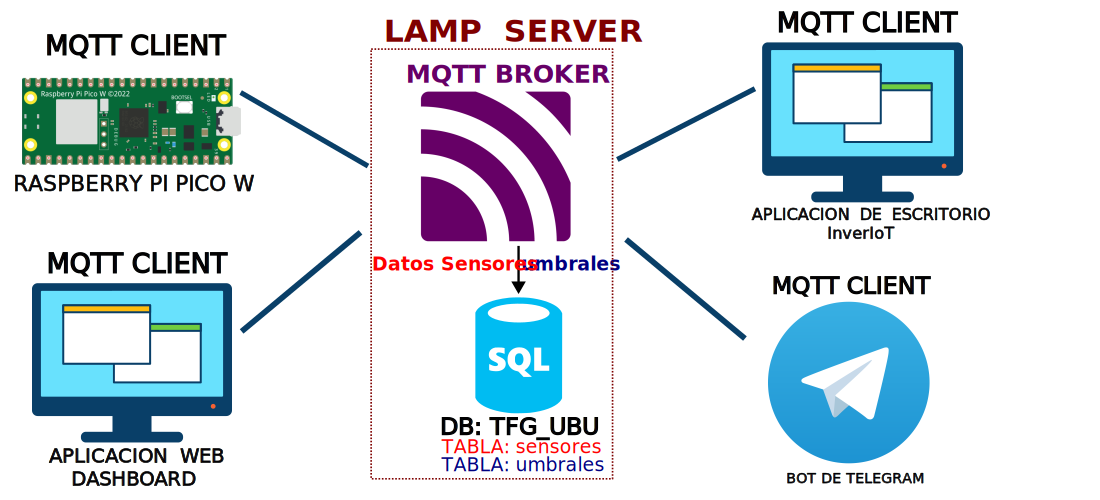
\includegraphics[width=1\textwidth]{img/diagramas/diagrama_general.png}
	\caption{Interacción entre cada parte del proyecto.} \label{Img:diagrama_general}
\end{figure}

Definimos umbrales (valor mínimo/máximo) para monitorizar cuando es que los valores de los sensores no están dentro de límites aceptables. En caso de detectar un valor anómalo fuera de estos umbrales, se genera una alerta.

\begin{table}[htbp]
\begin{center}
	\caption{Umbrales ideales para un invernadero de cannabis medicinal.}\label{tabla:umbrales}
\begin{tabular}{|l|l|l|l|}
\hline
\rowcolor[HTML]{C0C0C0} 
\textbf{Característica} & \textbf{Mínimo} & \textbf{Máximo} & \textbf{Unidades}\\ \hline
TEMPERATURA & 30 & 35 & \textcelsius\\ \hline
HUMEDAD & 30 & 70 & \% \\ \hline
LUMINOSIDAD & 30 & 150 & lux\\ \hline
HUMEDAD DEL SUELO & 20 & 80 & \% \\ \hline
\end{tabular}
\end{center}
\end{table}

%\begin{table}[htbp]
%\begin{center}
%\caption{Topics de MQTT usados.}
%\begin{tabular}{|l|l|} %|c|c|
%\hline
%\rowcolor[HTML]{C0C0C0} 
%\textbf{Nombre del topic} & \textbf{Descripción}\\ \hline
%invernadero/sensores & fecha, hora y valores de sensores \\ \hline
%invernadero/umbrales & valores límite \\ \hline
%invernadero/ordenes & Permite activar un mecanismo \\ \hline
%\end{tabular}
%\end{center}
%\end{table}

%A continuación veremos cada parte del proyecto para su mejor comprensión.

\subsection{Servidor LAMP}\label{proyecto:LAMP}

Opté por establecer un servidor LAMP para facilitar el envío y manejo de datos. La implementación de este servidor se llevó a cabo en el sistema operativo Ubuntu~\cite{misc:Ubuntu}, el cual fue virtualizado utilizando Hyper-V~\cite{manual:Hyper_V}.
En esta instancia, se emplea un servidor físico HP ProLiant~\cite{misc:HP_ProLiant} para la virtualización de los servicios Apache~\cite{misc:Apache}, MySQL~\cite{misc:Mysql}, PHP~\cite{misc:PHP} y SSH~\cite{misc:SSH}.

\begin{table}[htbp]
\begin{center}
\caption{Características del servidor HP ProLiant.}
\begin{tabular}{|l|l|}
\hline
\rowcolor[HTML]{C0C0C0} 
\textbf{Característica} & \textbf{Descripción}\\ \hline
Sistema operativo & Windows Server 2019 Standard\\ \hline
Fabricante & Hewlett Packard Enterprise \\ \hline
Modelo & Hewlett Packard Enterprise x64 Class PC\\ \hline
Procesador & Intel(R) Xeon(R) Silver 4210R CPU @ 2.4GHz 2.39GHz\\ \hline
Memoria instalada (RAM) & 128 GB (128 GB utilizable) \\ \hline
Tipo de sistema & Sistema operativo de 64 bits, procesador x64 \\ \hline
\end{tabular}
\end{center}
\end{table}

\begin{figure}[h]
	\centering
	\includegraphics[width=0.9\textwidth]{img/desarrollo/LAMP_servicios.png}
	\caption{Servicios instalados y operativos en el servidor LAMP.} \label{Img:LAMP_servicios}
\end{figure}

\subsection{NodeMqtt}\label{proyecto:NodeMqtt}

\textbf{NodeMqtt} es un servicio en Node.js~\cite{misc:Nodejs} que se ejecuta dentro del servidor LAMP, escucha los topics \textbf{invernadero/sensores} e \textbf{invernadero/umbrales}. Utiliza la librería MQTT.js~\cite{misc:MQTTjs}.

Está conformado por los siguientes archivos: index.js y package.json.

%\begin{itemize}
	%\item \textbf{index.js:}
		%Es el punto de entrada del código de la aplicación.
	%\item \textbf{package.json:}
		%Es un archivo de configuración que describe la aplicación y sus dependencias.
%\end{itemize}

Los datos son enviados por la placa Raspberry Pi Pico W RP2040~\cite{misc:RPiPicoW} usando MQTT, que recopila valores de sensores, y el servicio \textbf{nodeMqtt} captura los datos de los topics MQTT llamados \textbf{invernadero/sensores} e \textbf{invernadero/umbrales}, formatea y luego inserta estos datos en la base de datos MySQL~\cite{misc:Mysql} llamada \textbf{TFG\_UBU}.

La base de datos contiene dos tablas llamadas \textbf{sensores} y \textbf{umbrales}.

\begin{table}[htbp]
\begin{center}
	\caption{Columnas de las tablas contenidas en TFG\_UBU.}
\begin{tabular}{|l|l|}
\hline
\rowcolor[HTML]{C0C0C0} 
\textbf{sensores} & \textbf{umbrales}\\ \hline
fecha & temperatura\_minima \\ \hline
hora & temperatura\_maxima \\ \hline
temperatura & humedad\_ambiente\_minima \\ \hline
humedad & humedad\_ambiente\_maxima \\ \hline
intensidad\_luz & luminosidad\_minima \\ \hline
humedad\_suelo & luminosidad\_maxima \\ \hline
			   & humedad\_suelo\_minima \\ \hline
			   & humedad\_suelo\_maxima \\ \hline
			   & fecha\_actualización \\ \hline
\end{tabular}
\end{center}
\end{table}

\begin{figure}[h]
	\centering
	\includegraphics[width=1\textwidth]{img/diagramas/mqtt_nodeMqtt.png}
	\caption{MQTT con Node.js para almacenar datos de los sensores.}
\end{figure}

%\begin{figure}[h]
	%\centering
	%\includegraphics[width=0.1\textwidth]{img/desarrollo/mysql_tabla_sensores.png}
	%\caption{Data almacenada en la tabla \textbf{sensores}.}
%\end{figure}

\subsection{Hardware}\label{proyecto:Hardware}

Se optó por la Raspberry Pi Pico W debido a su eficiencia energética y coste accesible. Se conectaron al sistema un sensor de humedad y temperatura DHT22~\cite{manual:DHT22}, un sensor de intensidad de luz BH1750~\cite{manual:BH1750}, y un sensor de humedad de suelo~\cite{wiki:SensorHumedadSuelo}. Además, se incorporaron LEDs RGB~\cite{manual:LedRGB} para señalizar alertas.

\begin{figure}[h]
    \centering
    \includegraphics[width=1\textwidth]{img/diagramas/conexiones.png}
    \caption{Conexiones.} \label{Img:conexionesHardware}
\end{figure}

\begin{itemize}
	\item La Raspberry Pi Pico W estará situada en el invernadero para la recopilación de datos.
	\item Los LEDs RGB, instalados en la oficina del cliente, indicarán visualmente si los valores superan los umbrales establecidos.
	\item La pantalla OLED estará colocada en la puerta del invernadero para mostrar los valores actualizados.
\end{itemize}

Los datos se muestran en una pantalla OLED~\cite{manual:Oled} en tiempo real.

La Raspberry Pi Pico W establece conexión con el servidor LAMP a través de MQTT, facilitando la transmisión de los datos de los valores medidos por los sensores, el envío de umbrales predefinidos y la recepción de órdenes para ejecutar acciones específicas.

%\begin{figure}[h]
	%\centering
	%\includegraphics[width=0.5\textwidth]{img/fotos/conexiones_real.png}
	%\caption{Raspberry Pi Pico W y sensores conectados.} \label{Img:conexion_simple}
%\end{figure}

\begin{figure}[h]
	\centering
	\includegraphics[width=1\textwidth]{img/diagramas/mqtt_hardware.png}
	\caption{Conexión de la Raspberry Pi Pico W con el servidor LAMP.} \label{Img:mqtt_hardware}
\end{figure}

\begin{figure}[h]
	\centering
	\includegraphics[width=0.7\textwidth]{img/fotos/oled1.png}
	\caption{Pantalla oled conectada a la Raspberry Pi Pico W.} \label{Img:oled_conexion}
\end{figure}

%\begin{figure}[h]
	%\centering
	%\includegraphics[width=0.7\textwidth]{img/herramientas/rpipicow_umqtt.png}
	%\caption{Librería umqtt para conexión mediante MQTT.} \label{Img:rpipicow_umqtt}
%\end{figure}

\subsection{InverIoT}\label{proyecto:InverIoT}
Usando el lenguaje de programación C\#~\cite{manual:CSharp} y utilizando Windows Forms, se desarrolla una aplicación de escritorio para Windows al que se ha llamado InverIoT, que permite al usuario monitorizar el histórico de datos, y también visualizar los datos en tiempo real.

\begin{figure}[h]
    \centering
    \includegraphics[width=0.95\textwidth]{img/desarrollo/InverIoT_Desktop.png}
	\caption{Aplicación de escritorio \textbf{InverIoT}.}
\end{figure}

\begin{figure}[h]
    \centering
    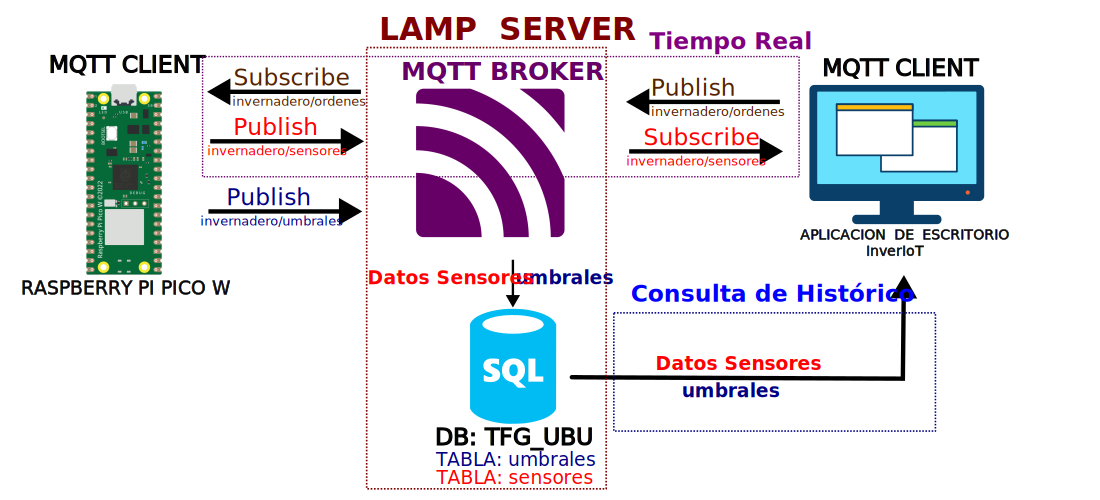
\includegraphics[width=1\textwidth]{img/diagramas/mqtt_InverIoT.png}
    \caption{Interacción entre la aplicación y el servidor LAMP.}
\end{figure}

Utilizando el protocolo MQTT~\cite{manual:MQTT}, la aplicación suscribe y recibe los datos publicados en el mismo tema. 

Para el histórico de datos no utiliza MQTT, se conecta al servidor LAMP mediante Mysql Protocol y extrae la data de la base de datos llamada \textbf{TFG\_UBU}.

\begin{figure}[h]
    \centering
    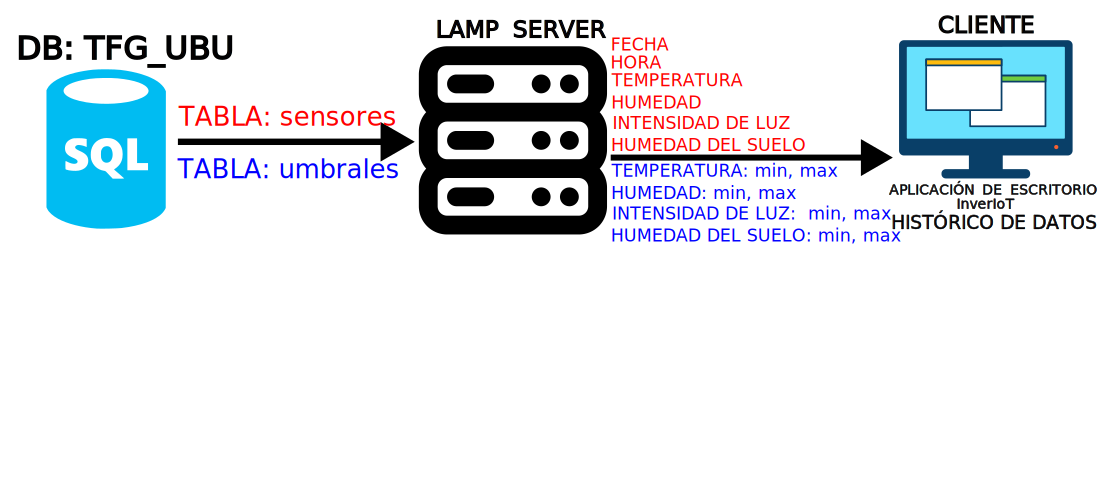
\includegraphics[width=1\textwidth]{img/diagramas/mqtt_InverIoT_Historico.png}
    \caption{Datos usados para mostrar el histórico de datos.}
\end{figure}


Estos datos son formateados y presentados en textboxes correspondientes, con unidades de medida agregadas.

Se incorporan botones para activar o desactivar mecanismos, esto es representado prendiendo o apagando un LED verde, recordar que hay un led RGB por cada variable medida.


\begin{figure}[h]
    \centering
    \includegraphics[width=1\textwidth]{img/desarrollo/InverIoT_Desktop_botones_control.png}
	\caption{Botones para activar o desactivar mecanismos.}
\end{figure}

\begin{figure}[h]
	\centering
	\includegraphics[width=0.85\textwidth]{img/desarrollo/InverIoT_verde_clickMecanismo.png}
	\caption{Activación de un mecanismo mediante un clic.}\label{img:InverIoTBotones}
\end{figure}

\begin{figure}[h]
	\centering
	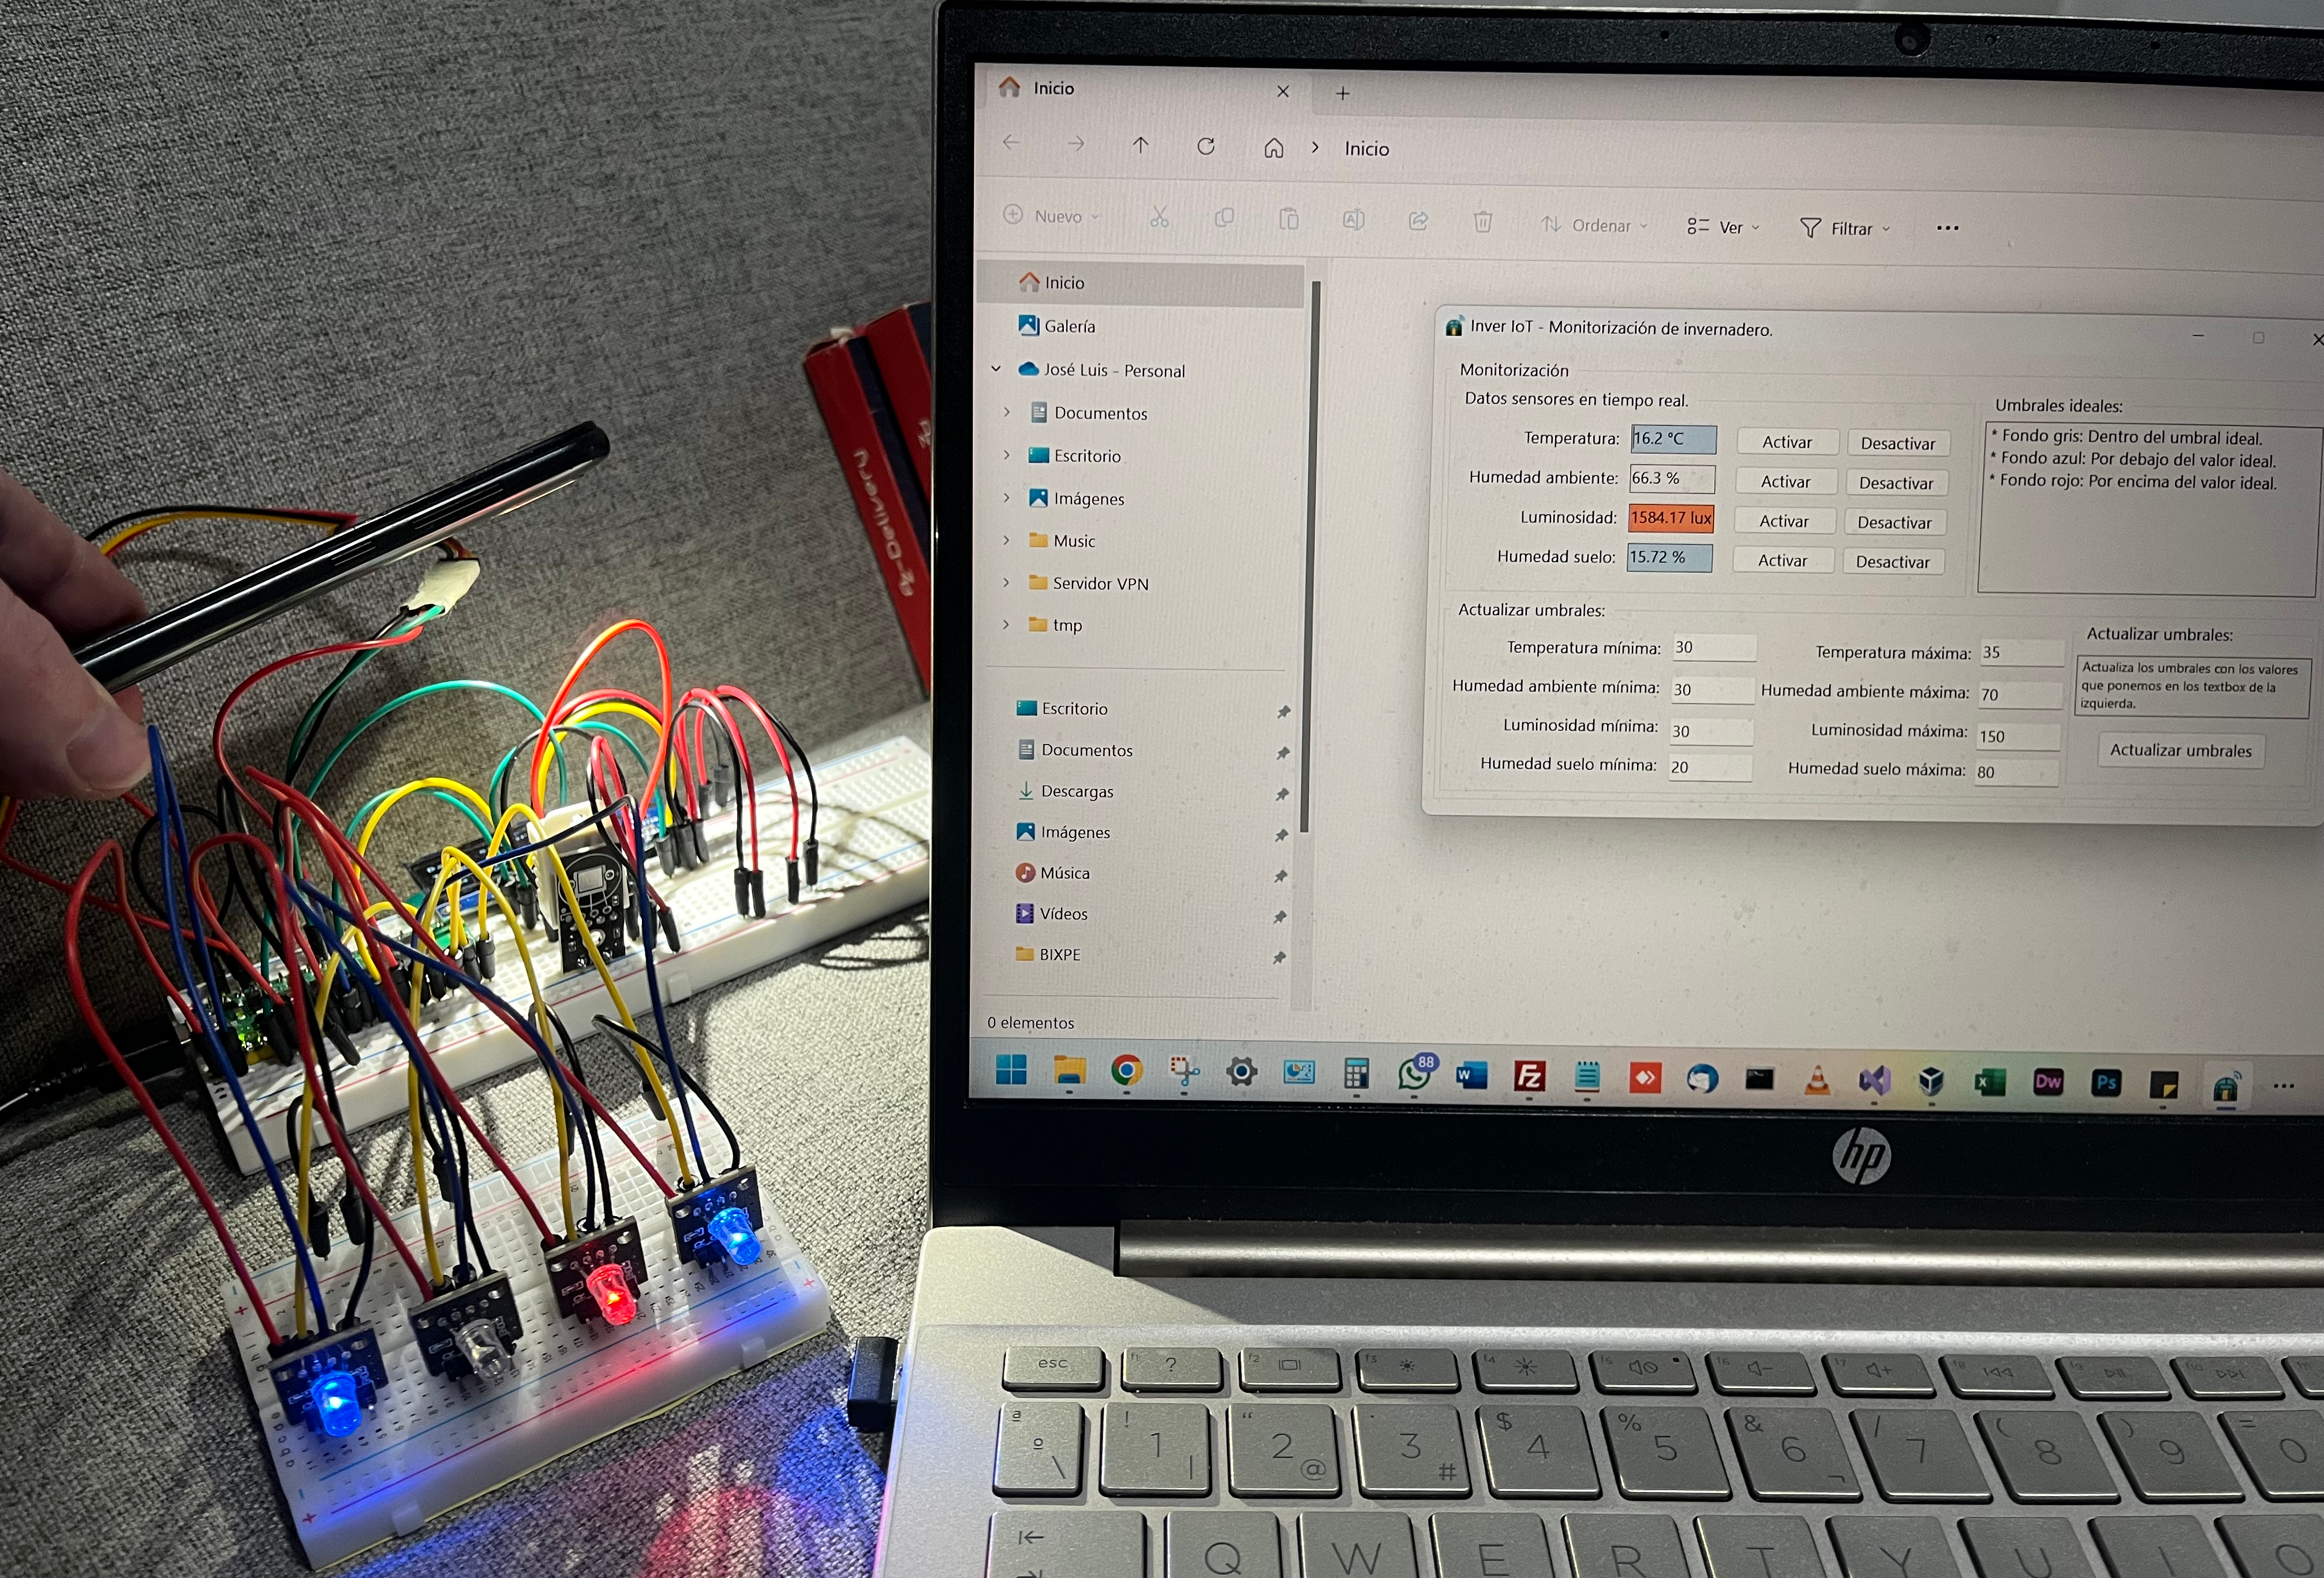
\includegraphics[width=0.85\textwidth]{img/fotos/InverIoT_PasandoUmbralLuz.png}
	\caption{Aplicación indicando que se ha sobrepasado el umbral de luz.}\label{img:InverIoTPasandoUmbralLuz}
\end{figure}

En la imagen \ref{img:InverIoTBotones} se puede observar 8 textboxes en la parte inferior para ajustar manualmente los valores mínimos y máximos de cada parámetro. Inicialmente estos valores fueron extraídos de la base de datos en el servidor LAMP.

En la imagen \ref{img:InverIoTPasandoUmbralLuz} se está sometiendo al sensor de intensidad de luz a sobrepasar el umbral establecido, el led rojo indica eso. Si un valor está por debajo del umbral, se indicará mediante el led de color azul. Se puede observar tal acontecimiento de colores en el hardware y en la aplicación de escritorio.

\begin{figure}[h]
    \centering
    \includegraphics[width=0.95\textwidth]{img/desarrollo/InverIoT_Histórico.png}
    \caption{Historial de los datos mostrada en la aplicación.}
\end{figure}


\begin{figure}[h]
    \centering
    \includegraphics[width=0.95\textwidth]{img/desarrollo/InverIoT_Gráficas.png}
    \caption{Gráfica mostrando los datos en un intervalo de fechas.}
\end{figure}




\pagebreak

\subsection{Dashboard}\label{proyecto:Dashboard}
Se ha creado un dashboard web con Node.js que habilita al usuario para visualizar en tiempo real los datos capturados por los sensores y acceder a un historial con filtro de fecha. La interfaz presenta similitudes con la aplicación de escritorio para mantener una experiencia coherente.

Los valores que exceden los umbrales establecidos se destacan mediante cambios de color.

\begin{figure}[h]
    \centering
    \includegraphics[width=0.95\textwidth]{img/desarrollo/Dashboard1.png}
    \caption{Intensidad de luz superando los umbrales.} \label{Img:Dashboard1}
\end{figure}

La plataforma incluye una gráfica en tiempo real y la capacidad de acceder a un historial con filtro de fecha.

\begin{figure}[h]
    \centering
    \includegraphics[width=0.95\textwidth]{img/diagramas/mqtt_dashboard.png}
    \caption{Dashboard web interactuando con el servidor LAMP.} \label{Img:mqtt_dashboard}
\end{figure}

La imagen \ref{Img:mqtt_dashboard} ilustra de manera significativa el uso de MQTT para la obtención de datos en tiempo real. Cabe destacar que, además, se utiliza el protocolo MySQL para extraer información de la base de datos alojada en el servidor LAMP, permitiendo así mostrar el histórico de datos

\begin{figure}[h]
    \centering
    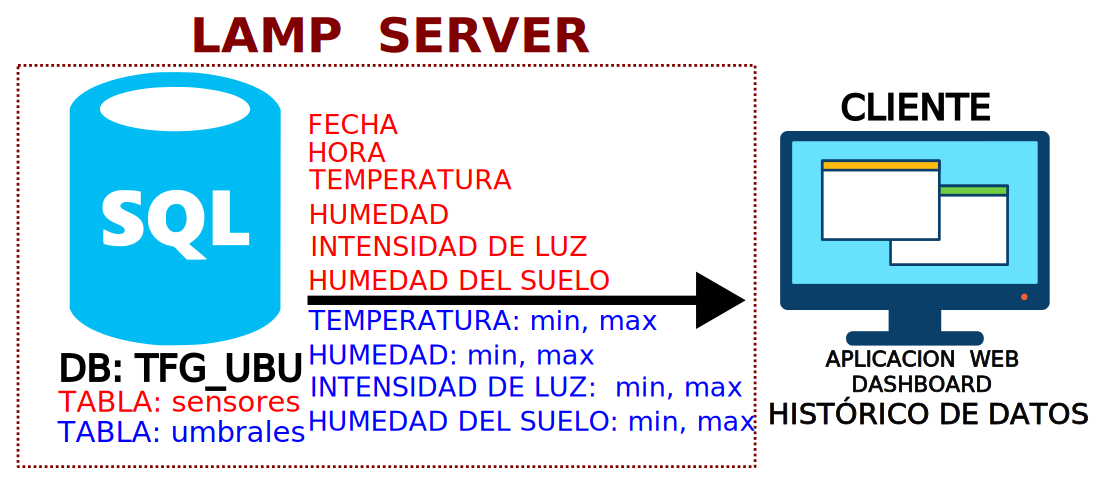
\includegraphics[width=1\textwidth]{img/diagramas/mqtt_dashboard_Historico.png}
    \caption{Valores específicos extraídos de la base de datos.} \label{Img:Dashboard_diagrama_Historico}
\end{figure}

\begin{figure}[h]
    \centering
    \includegraphics[width=0.95\textwidth]{img/desarrollo/Dashboard_Historico.png}
    \caption{Vista del historial, al cargar, muestra los datos del día actual.} \label{Img:Dashboard_Historico}
\end{figure}

%\begin{figure}[h]
    %\centering
    %\includegraphics[width=1\textwidth]{img/diagramas/mqtt_dashboard_TiempoReal.png}
    %\caption{Mediante MQTT extrae los datos para mostrarlos en tiempo real.} \label{Img:Dashboard_diagrama_TiempoReal}
%\end{figure}

El panel de control está disponible para su acceso a través del siguiente enlace: \href{http://www.inveriot.com}{InverIoT Dashboard}


%\begin{figure}[h]
	%\centering
	%\includegraphics[width=1\textwidth]{img/desarrollo/Dashboard2.png}
	%\caption{Página Web \href{http://www.inveriot.com}{InverIoT} desarrollada con Node.js.}
%\end{figure}

%\begin{figure}[h]
	%\centering
	%\includegraphics[width=1\textwidth]{img/desarrollo/Dashboard3.png}
	%\caption{Página Web \href{http://www.inveriot.com}{InverIoT} desarrollada con Node.js.}
%\end{figure}
%En este contexto, detallaré la configuración del servidor y la implementación de Node.js en la página web.

\subsection{Bot de Telegram}\label{proyecto:BotTelegram}

Se implementó la funcionalidad de enviar alertas a través de Telegram en caso de que los valores recopilados excedieran los umbrales ideales~\ref{tabla:umbrales}.

Para esta función, empleamos un bot de Telegram~\cite{misc:Telegram_bots} que envía mensajes de alerta si alguno de los valores está fuera del umbral establecido. 

La creación del bot se hace utilizando BotFather\cite{misc:BotFather} que es un bot especial en la plataforma de mensajería Telegram~\cite{misc:Telegram} que permite a los usuarios crear y gestionar sus propios bots. Al interactuar con BotFather, los usuarios pueden definir el nombre, la descripción, la imagen y otras configuraciones de su bot. Además, BotFather proporciona un token único para cada bot creado, el cual se utiliza para autenticar las solicitudes y permitir la interacción entre el bot y la plataforma de Telegram.

Para este proyecto el nombre del bot creado es \textbf{InverIoTBot}.

\begin{figure}[h]
	\centering
	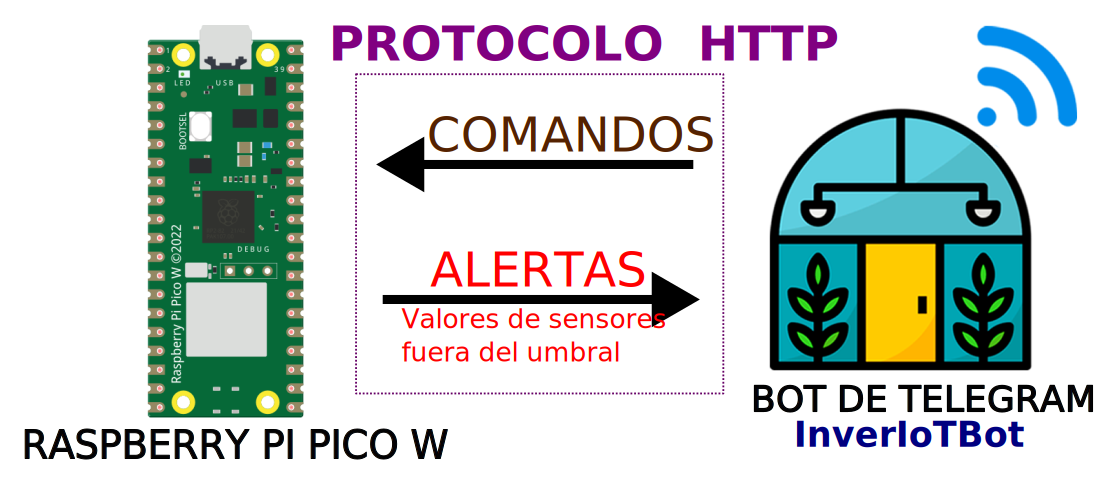
\includegraphics[width=1\textwidth]{img/diagramas/telegramBot.png}
	\caption{La interacción es mediante protocolo HTTP.} \label{Img:telegramBot}
\end{figure}

El bot también brinda la posibilidad de enviar comandos para acciones específicas, como obtener el valor de un sensor o activar un mecanismo vinculado a un sensor en particular.

Tener presente que la activación de un mecanismo se representa encendiendo un LED de color verde, y cada sensor está asociado a un LED RGB específico.
 
\begin{table}[htbp]
\begin{center}
\caption{Comandos del bot para la consulta de los datos.}
\begin{tabular}{|l|l|} %|c|c|
\hline
\rowcolor[HTML]{C0C0C0} 
\textbf{Comando} & \textbf{Valor que retorna}\\ \hline
/temp & Temperatura del ambiente\\ \hline
/huma& Humedad del ambiente \\ \hline
/lum & Luminosidad\\ \hline
/hums & Humedad del suelo\\ \hline
/todos & Todos los valores de los sensores\\ \hline
\end{tabular}
\end{center}
\end{table}


\begin{table}[htbp]
\begin{center}
\caption{Comandos del bot para activar un mecanismo.}
\begin{tabular}{|l|l|} %|c|c|
\hline
\rowcolor[HTML]{C0C0C0} 
\textbf{Comando} & \textbf{Acción específica}\\ \hline
/t\_ON & Mecanismo de temperatura prendido\\ \hline
/t\_OFF & Mecanismo de temperatura apagado\\ \hline
/ha\_ON & Mecanismo de humedad del ambiente prendido\\ \hline
/ha\_OFF & Mecanismo de humedad del ambiente apagado\\ \hline
/l\_ON & Mecanismo de luminosidad prendido\\ \hline
/l\_OFF & Mecanismo de luminosidad apagado\\ \hline
/hs\_ON & Mecanismo de humedad del suelo prendido\\ \hline
/hs\_OFF & Mecanismo de humedad del suelo apagado\\ \hline
\end{tabular}
\end{center}
\end{table}

\begin{figure}[h]
	\centering
	\includegraphics[width=0.7\textwidth]{img/desarrollo/BotTelegram_alertas.png}
	\caption{Alertas del bot de Telegram.} \label{Img:BotTelegram_alertas}
\end{figure}

\begin{figure}[h]
	\centering
	\includegraphics[width=0.7\textwidth]{img/desarrollo/BotTelegram_comandos.png}
	\caption{Consulta a la base de datos mediante comandos usando Telegram.}
\end{figure}

\capitulo{6}{Trabajos relacionados}

Para comprender plenamente la contribución y novedad de este proyecto, es esencial explorar investigaciones y desarrollos previos relacionados.

\subsection{Monitorización de la energía consumida mediante Raspberry Pi para sistema domótico}\label{Proy1}

Se trata de un TFG desarrollado en la Universidad Carlos III de Madrid que trata sobre un sistema de monitorización de energía consumida para una instalación domótica mediante el uso de una Raspberry Pi, en el que se debe realizar el diseño del circuito y la programación correspondientes para poder extraer datos de diez sensores de corriente de forma simultánea.

Cada sensor recoge información correspondiente a una línea del cuadro de electricidad donde irá instalado.

En el desarrollo de este proyecto se pueden diferenciar dos partes:

\begin{itemize}
\item Montaje del circuito que lleva los datos obtenidos de los sensores de corriente hacia la Raspberry Pi para que puedan ser gestionados adecuadamente.

\item Configuración de la Raspberry Pi para la lectura y procesado de los datos obtenidos a través de cada uno de los sensores. Tales datos son guardados en diferentes ficheros dependiendo del canal de los que provengan, denominados datos\_canalX.txt, donde X es el número del sensor.
\end{itemize}

Introduciendo un comando determinado el sistema es capaz de:

\begin{itemize}
	\item Modificar el tiempo existente entre el recojo de cada muestra para un canal específico, que es guardado en un fichero de tiempos para su continua lectura.
	\item Recoger datos a partir de un canal, fecha y hora, de forma que se lee el fichero datos\_canalX correspondiente al canal introducido, y se guardan en otro fichero todos aquellos datos posteriores a la fecha y hora introducidos.
\end{itemize}

Podemos ver su referencia en la bibliografía en la referencia~\cite{TesisBaron2017}.

En la columna \textbf{Proy1} de la tabla~\ref{tabla:comparativa-proyectos} podemos ver algunas características de este proyecto.

\subsection{Diseño e implementación de un sistema domótico basado en Raspberry Pi}\label{Proy2}

Se trata de un TFG desarrollado en la Universidad Carlos III de Madrid que trata sobre un sistema domótico de bajo coste, basado en código libre (UNIX/LINUX). Dicho sistema permite al usuario manejar de forma fácil y sencilla elementos finales como motores y leds.

El elemento de software principal es el sistema operativo Raspbian (basado en Debian), aunque ahora es llamado Raspberry Pi OS. Tal sistema operativo es instalado en la RaspberryPi.

El segundo elemento software importante es el servidor web Apache que gestiona la aplicación web desarrollada bajo el patrón de desarrollo Modelo-Vista-Controlador (MVC).

El sistema domótico está compuesto por varios sus-sistemas:

\begin{itemize}
	\item La aplicación web.
	\item La base de datos.
	\item El conjunto de sensores y actuadores.
\end{itemize}

La aplicación web se ha desarrollado sobre un servidor LAMP que es accesible desde el exterior y que actua de interfaz sobre el usuario del sistema domótico y le propio sistema.

Algunas acciones que puede realizar el usuario mediante este sistema:

\begin{itemize}
	\item Consultar temperatura y humedad.
	\item Controlar apertura puertas/persianas.
	\item Consultar histórico de temperaturas y humedades.
	\item Consultar movimiento en una habitación.
	\item Controlar iluminación interior.
\end{itemize}

Podemos ver su referencia en la bibliografía en la referencia~\cite{TesisSantos2017}.

En la columna \textbf{Proy2} de la tabla~\ref{tabla:comparativa-proyectos} podemos ver algunas características de este proyecto.

\section{Fortalezas y debilidades este proyecto}

Las fortalezas clave del proyecto son:

\begin{itemize}
	\item Todos los elementos utilizados en este proyecto son fácilmente accesibles, tanto en términos de software como de hardware.
	\item La elección de la Raspberry Pi Pico W fue crucial gracias a su bajo consumo de energía, su compacto tamaño que facilita la portabilidad y su capacidad de conectividad Wifi.
	\item La versatilidad de la Raspberry Pi Pico W, con su capacidad de conectividad Wifi, ha posibilitado tanto el envío de datos como la recepción de órdenes. Además, su flexibilidad se evidencia en la implementación exitosa de MQTT en el proyecto.
	\item La modularidad del sistema permite una fácil escalabilidad, ya que es posible agregar nuevos sensores o funcionalidades sin mayores complicaciones.		
	\item La presentación gráfica de datos en tiempo real en una pantalla OLED y la posibilidad de acceder a través de una aplicación de escritorio y un panel web ofrecen múltiples formas de acceder y visualizar la información recopilada.
\end{itemize}

Las principales debilidades de este proyecto son:

\begin{itemize}
	\item La prueba del sistema se realizó en un ambiente no controlado, lo que puede afectar la precisión de los datos y la generación de alertas. Esto podría limitar la fiabilidad de las respuestas del sistema en condiciones reales.
	\item La funcionalidad del proyecto está intrínsecamente ligada a la conectividad Wifi de la Raspberry Pi Pico W. Problemas en la red Wifi podrían afectar la transmisión de datos y la recepción de órdenes.
	\item Aunque se han incluido sensores relevantes, la variedad podría ser limitada. La adición de más tipos de sensores podría mejorar la capacidad de monitoreo y la precisión de los datos recopilados.
	\item A medida que se agregan más sensores y funcionalidades, la capacidad de la Raspberry Pi Pico W podría alcanzar sus límites. En proyectos a mayor escala, se podría requerir hardware más potente.
\end{itemize}

\begin{table}[htbp]
\centering
\begin{tabular}{lccc}
\toprule
Características & MICM & Proy1 & Proy2  \\
\midrule
Proyecto libre & \cellcolor{green!25} {\checkmark} & \cellcolor{green!25} {\checkmark} & \cellcolor{green!25} {\checkmark} \\
Menor precio en modelo de Raspberry Pi & \cellcolor{green!25} {\checkmark} & \cellcolor{red!25} {\xmark} & \cellcolor{red!25} {\xmark} \\
Menor consumo de energía de Raspberry Pi & \cellcolor{green!25} {\checkmark} & \cellcolor{red!25} {\xmark} & \cellcolor{red!25} {\xmark} \\
Escalabilidad & \cellcolor{green!25} {\checkmark} & \cellcolor{green!25} {\checkmark} & \cellcolor{green!25} {\checkmark} \\
Modularidad & \cellcolor{green!25} {\checkmark} & \cellcolor{green!25} {\checkmark} & \cellcolor{green!25} {\checkmark} \\
Más opciones de visualización de datos & \cellcolor{green!25} {\checkmark} & \cellcolor{red!25} {\xmark} & \cellcolor{red!25} {\xmark} \\
Mayor potencia en modelo de Raspberry Pi & \cellcolor{red!25} {\xmark} & \cellcolor{green!25} {\checkmark} & \cellcolor{green!25} {\checkmark} \\
Más opciones de acceso de datos & \cellcolor{green!25} {\checkmark} & \cellcolor{red!25} {\xmark} & \cellcolor{red!25} {\xmark} \\
Interacción multiplataforma             & \cellcolor{green!25} {\checkmark} & \cellcolor{green!25} {\checkmark} & \cellcolor{green!25} {\checkmark} \\
WiFi entre elementos                    & \cellcolor{green!25} {\checkmark} & \cellcolor{green!25} {\checkmark} & \cellcolor{green!25} {\checkmark \\
Almacenamiento de datos                    & \cellcolor{green!25} {\checkmark} & \cellcolor{green!25} {\checkmark} & \cellcolor{green!25} {\checkmark} \\
\bottomrule
\end{tabular}
\caption{Comparativa de las características de los proyectos.}
\label{tabla:comparativa-proyectos}
\end{table}

%Este apartado sería parecido a un estado del arte de una tesis o tesina. En un trabajo final grado no parece obligada su presencia, aunque se puede dejar a juicio del tutor el incluir un pequeño resumen comentado de los trabajos y proyectos ya realizados en el campo del proyecto en curso. 

\capitulo{7}{Conclusiones y Líneas de trabajo futuras}

Con esta sección, finaliza la documentación del proyecto, detallando los objetivos alcanzados. A continuación, se presentarán algunas posibles direcciones para investigaciones futuras que podrían ampliar y mejorar significativamente el proyecto.

\section{Conclusiones}

Al concluir el proyecto, podemos afirmar lo siguiente:

\begin{itemize}
\item Se lograron alcanzar los objetivos establecidos al inicio del proyecto, los cuales se centraban en la recopilación y visualización de datos ambientales en invernaderos de cannabis medicinal.
\item La elección de la Raspberry Pi Pico W demostró ser acertada, ya que su bajo consumo de energía, tamaño compacto y conectividad WiFi facilitaron la implementación a un costo razonable.
\item Tanto los componentes hardware como el software seleccionados son de fácil adquisición, permitiendo replicar el sistema con relativa facilidad. Esto contribuye a la accesibilidad de la tecnología en el ámbito de los invernaderos.
\item La capacidad de conectividad WiFi de la Raspberry Pi Pico W permitió la transmisión de datos y la recepción de órdenes de manera eficiente. La implementación de MQTT agregó una capa adicional de versatilidad al sistema.
\item Se logró una amplia variedad de formas de visualizar los datos ambientales, proporcionando a los usuarios una comprensión más completa y detallada de las condiciones dentro del invernadero.
\item Se identifican oportunidades para futuras mejoras, como la expansión de la capacidad de monitoreo, la integración de más sensores especializados y la implementación de alertas automáticas ante condiciones críticas.
\item Este proyecto brinda una solución económica y accesible para invernaderos de cannabis medicinal, con potencial para adaptarse a otros entornos de cultivo.
\end{itemize}

\section{Líneas de trabajo futuras}

El proyecto se ha desarrollado de manera integral, abordando de manera efectiva la funcionalidad deseada y proporcionando una solución adecuada a las necesidades planteadas. Aunque se ha logrado un producto sólido, existe el potencial para mejorar en diversos aspectos. 

\begin{itemize}
\item Integrar sensores adicionales para monitorizar parámetros específicos del entorno del invernadero, como la concentración de CO2, la calidad del suelo, o la presencia de plagas. Esto proporcionaría un monitoreo más completo y detallado.
\item Desarrollar algoritmos de análisis de datos más avanzados para identificar patrones, tendencias o anomalías en la información recopilada. Esto proporcionaría insights más profundos sobre el comportamiento del invernadero.
\item Mejorar la interfaz de usuario para proporcionar funcionalidades más avanzadas, gráficos interactivos, información estadística y herramientas de análisis. Esto facilitaría la interpretación de los datos y la toma de decisiones.
\item Integrar un sistema de riego automatizado que pueda ajustarse en tiempo real según las condiciones ambientales registradas. Esto optimizaría el consumo de agua y mejoraría la eficiencia del proceso de cultivo.
\item Extender las pruebas y adaptar el sistema para su uso en otros tipos de cultivos, permitiendo su aplicación en entornos agrícolas más amplios.
\item Reforzar la seguridad del sistema, incluyendo medidas para proteger la integridad de los datos y garantizar la privacidad de la información recopilada.
\end{itemize}

%Todo proyecto debe incluir las conclusiones que se derivan de su desarrollo. Éstas pueden ser de diferente índole, dependiendo de la tipología del proyecto, pero normalmente van a estar presentes un conjunto de conclusiones relacionadas con los resultados del proyecto y un conjunto de conclusiones técnicas. 
%Además, resulta muy útil realizar un informe crítico indicando cómo se puede mejorar el proyecto, o cómo se puede continuar trabajando en la línea del proyecto realizado. 


\bibliographystyle{plain}
\bibliography{bibliografia}

\end{document}
